\documentclass[12pt,a4paper,ngerman]{article}
\usepackage{stylesheet}
\begin{document}
\TUHeader                          %  Bitte Ausfüllen!!!
%----------------------------
{Übung F: Übertragungsverhalten nachrichtentechnischer Systeme}                       %  Übungstitel
%----------------------------
{25.11.2014}                        %  Übungsdatum
%----------------------------
{05}                            %  Gruppen-Nr.
%----------------------------
{Thomas Neff}                   % Name des Protokollführers
%----------------------------
{
1.~Daniel Freßl, 1230028\\
2.~Thomas Neff, 1230319\\                    %  Übungsteilnehmer
3.~Thomas Pichler, 1230320 \\                   %  ...bei <4 Teilnehmer auskommentieren
4.~Martin Winter, 1130688\\
5.~Bernadette Schreyer, 1073076\\
}
%----------------------------
{Ao.Univ.-Prof. Dipl.-Ing. Dr. techn. Erich Leitgeb}
{Max Henkel}                          %  Betreuer
%----------------------------
{Graz}                              %  Ort der Protokollerstellung
{\today}                            %  Datum Protokollerstellung




\pagebreak
  
\tableofcontents
  
\pagebreak

%-------------------------------------------------------------------------------
%
% Beginn des Protokolls
%
%-------------------------------------------------------------------------------

\section{Demodulation eines QPSK-Signals mit unbekannten Paramteren}
\subsection{Aufgabenstellung}
Gegeben ist ein Signal, welches mittels QPSK auf einen HF-Träger moduliert wurde. Sie sollen dieses Signal nun mit dem in der Software integrierten digitalen Demodulator demodulieren. Da Ihnen die Paramter Trägerfrequenz, Symbolrate und senderseitig verwendetes Filter unbekannt sind, müssen Sie diese bestimmen.
\begin{itemize}
\item Bestimmen Sie die Trägerfrequenz und stellen Sie das Signal in Frequenz- und Zeitbereich sinnvoll dar. 
\item Bestimmen Sie die Symbolrate. Versuchen Sie dazu die Darstellung des Spektrums zu glätten.
\item Bestimmen Sie anhand des Spektrums den Filtertyp und dessen Parameter.
\item Demodulieren Sie das Signal. Stellen Sie Konstellations- und Augendiagramm sowie das Spektrum des Signals dar. 
\item Woran ist erkennbar, dass der richtige Filtertyp gefunden wurde. Überprüfen Sie ihre Antwort durch Veränderung der Einstellungen
\end{itemize}
\cite[18]{skript}

\subsection{Messaufbau}
Es wurde kein Messaufbau benötigt.
\subsection{Tabellen}
Es waren keine Tabellen aufzunehmen. 
\subsection{Formeln}
Die Symbolrate bei QPSK ergibt sich zu
\begin{equation}
f_N = \frac{f_S}{2} \quad \Rightarrow \quad f_S = 2 \cdot f_N
\end{equation}
Die absolute Bandbreite ergibt sich durch
\begin{equation}
B = B_N (1+\alpha)
\end{equation}
\pagebreak
\subsection{Berechnungsbeispiele}
Aus der Nyquistfrequenz $f_N$ lässt sich die Symbolrate bestimmen
\begin{equation}
f_N = \frac{f_S}{2} \Rightarrow f_S = 2 \cdot f_N
\end{equation}
Mit $f_N = 5$ MHz lässt sich $f_S$ somit bestimmen als
\begin{equation}
f_S = 2 \cdot f_N = 2 \cdot 5 \text{ MHz} = 10 \text{ MHz}
\end{equation}
Aus der Kenntnis der absoluten Bandbreite $B = 19$ MHz und der Nyquistbandbreite \\ $B_N = 2 \cdot f_N = 2 \cdot 5 \text{ MHz} = 10$ MHz lässt sich der Roll-off Faktor $\alpha$ bestimmen
\begin{equation}
B = B_N(1+\alpha) = 19 \text{ MHz} \quad \Rightarrow \quad \alpha = \frac{B}{B_N} -1 = \frac{19 \text{ MHz}}{10 \text{ MHz}} -1 = 0.9
\end{equation}



\subsection{Diagramme}
\begin{figure}[H]
\centering
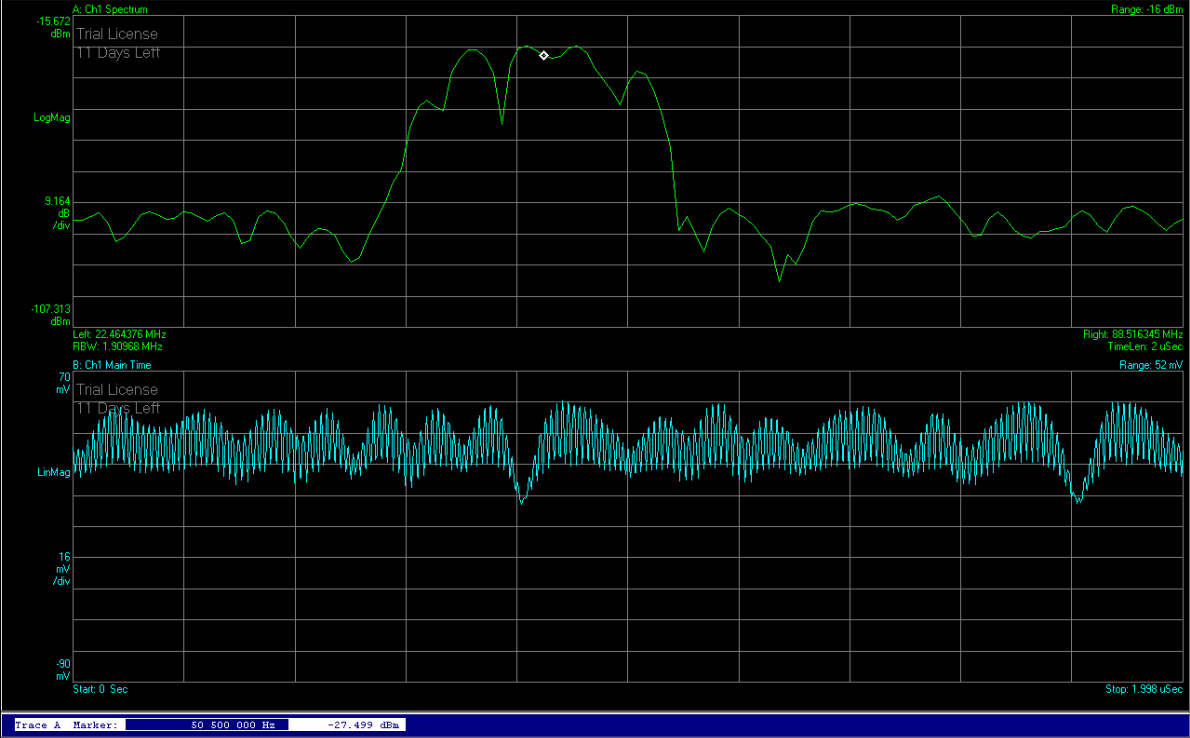
\includegraphics[width=0.9\textwidth]{figures/Aufgabe1_QPSK.jpg} 
\caption{Signal in Frequenz- und Zeitbereich}
\label{fig:1_sig}
\end{figure}


\begin{figure}[H]
\centering
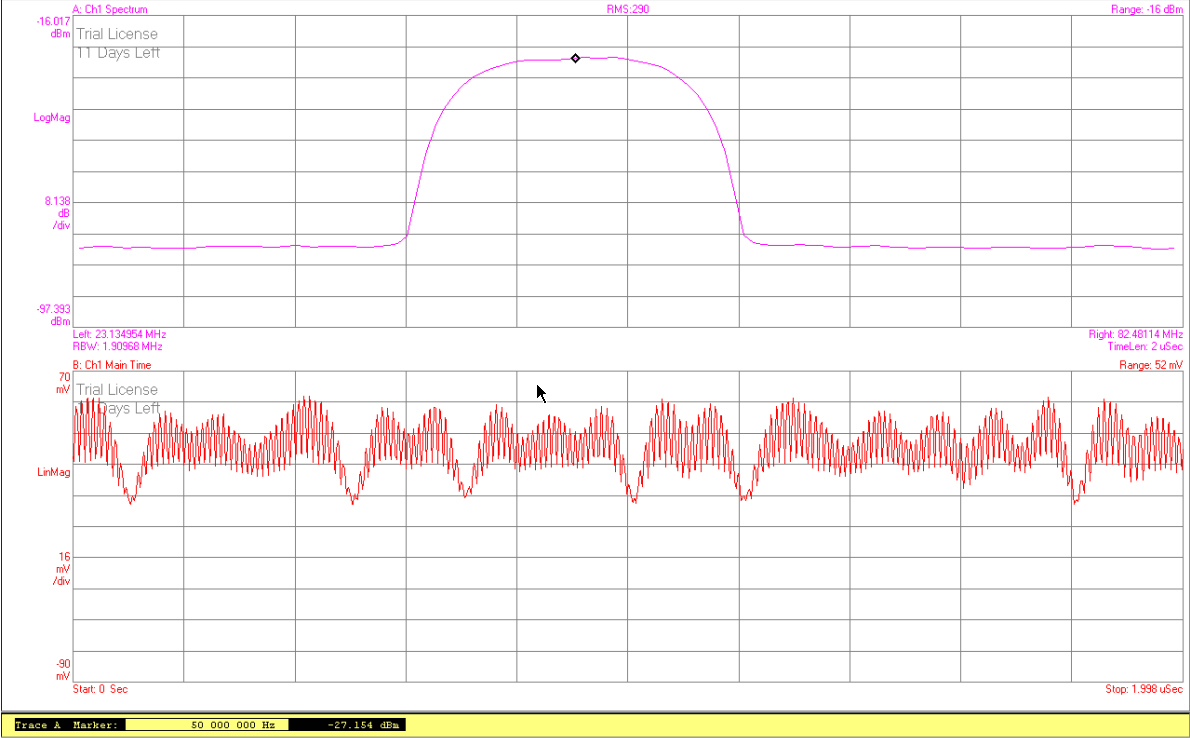
\includegraphics[width=0.9\textwidth]{figures/Aufgabe1_QPSK_avg.jpg} 
\caption{Signal geglättet in Frequenz- und Zeitbereich}
\label{fig:1_sig_avg}
\end{figure}



\begin{figure}[H]
\centering
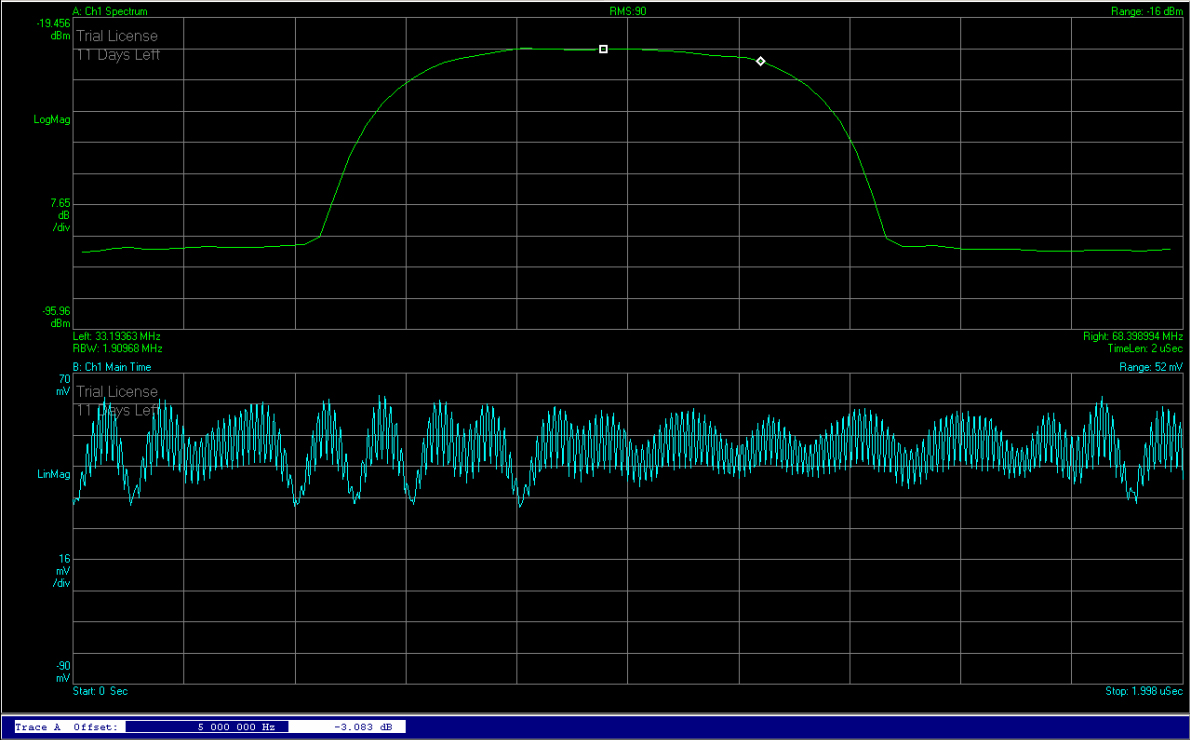
\includegraphics[width=0.9\textwidth]{figures/Aufgabe1_QPSK_fs.jpg} 
\caption{Ermittelung von $f_N$ mittels Software-Marker}
\label{fig:1_fn}
\end{figure}

\pagebreak

\begin{figure}[H]
\centering
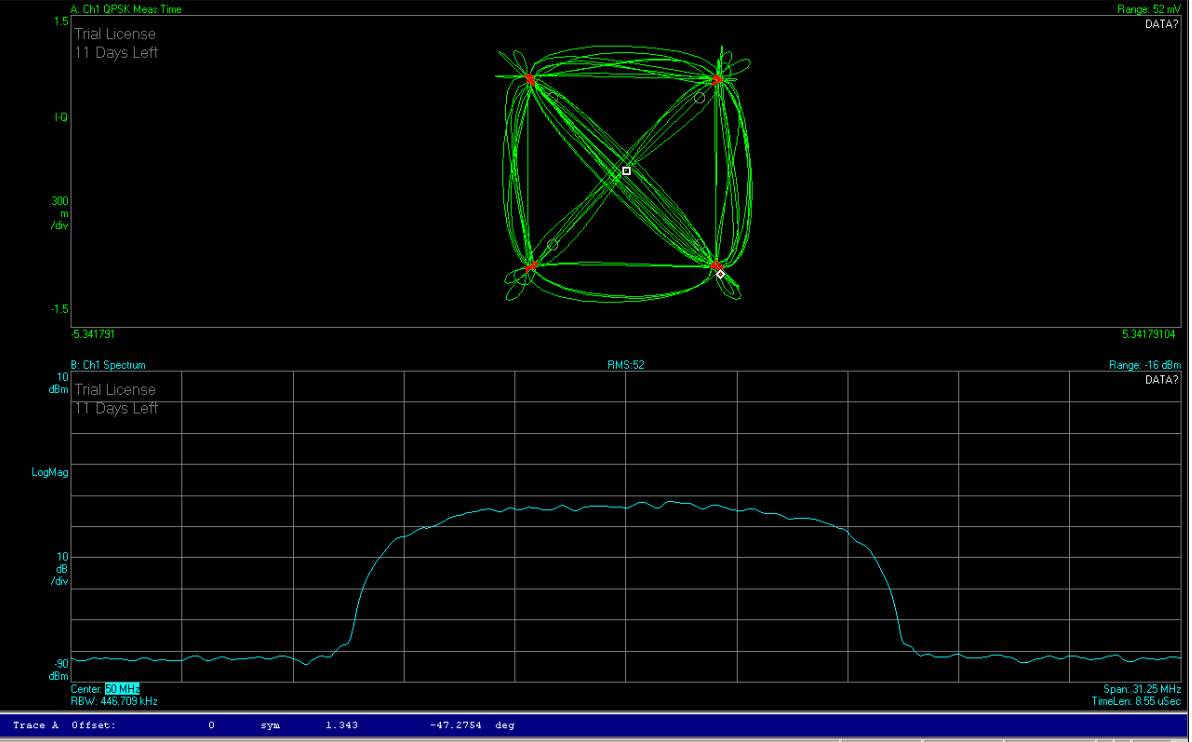
\includegraphics[width=0.9\textwidth]{figures/Aufgabe1_QPSK_demod.jpg} 
\caption{Konstellationsdiagramm des Signals}
\label{fig:1_konst}
\end{figure}


\begin{figure}[H]
\centering
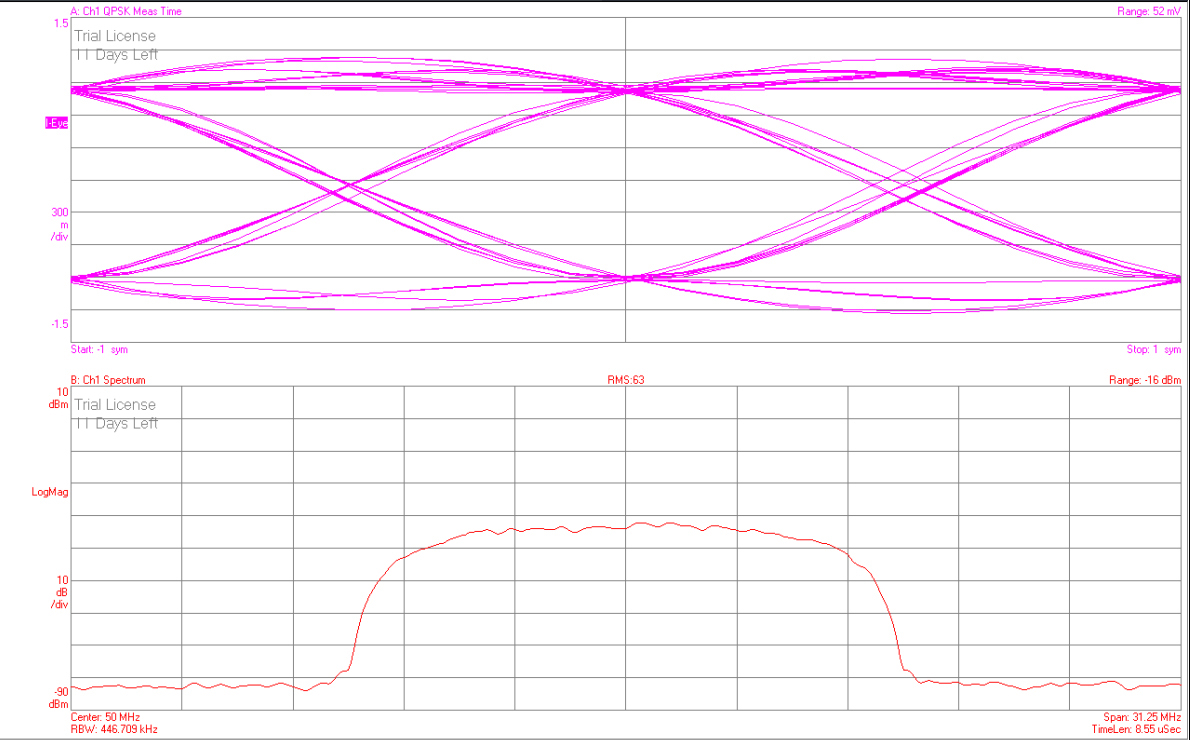
\includegraphics[width=0.9\textwidth]{figures/Aufgabe1_QPSK_demod_i_eye.jpg} 
\caption{Augendiagramm des Signals}
\label{fig:1_auge}
\end{figure}

\pagebreak

\begin{figure}[H]
\centering
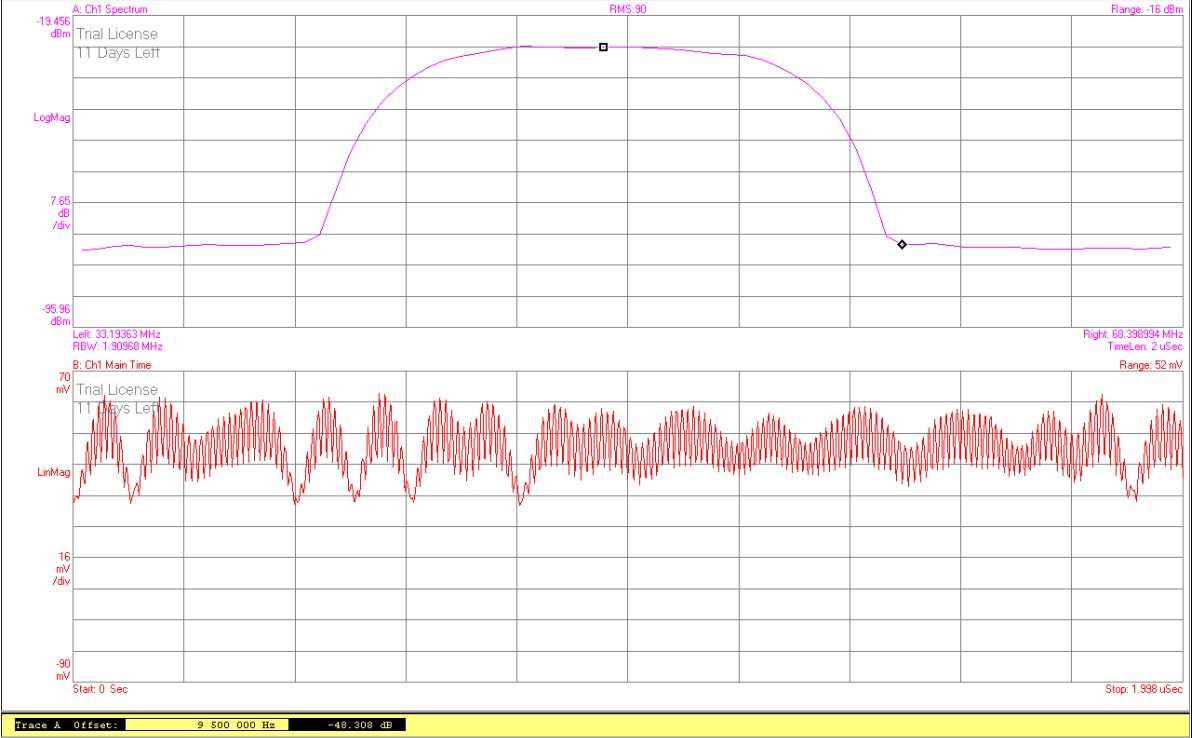
\includegraphics[width=0.9\textwidth]{figures/Aufgabe1_QPSK_B.jpg} 
\caption{Ermittlung von $B_N$ mittels Software-Marker}
\label{fig:1_bn}
\end{figure}



\subsection{Diskussion}
Gegeben war ein mittels QPSK auf einen HF-Träger moduliertes, breitbandiges Signal, welches mit der Software \textit{Agilent 89600 Vector Signal Analysis Software} demoduliert werden sollte. In Abbildung \ref{fig:1_sig} sieht man das Signal. Um Aussagen und Messungen zu erleichtern, wurde das Signal in Software mit den Einstellungen \textit{Average Type RMS (Video)} und \textit{Count 100} \cite[23]{skript} geglättet, dies führt zu Abbildung \ref{fig:1_sig_avg}. \\
Somit lies sich dann die Trägerfrequenz in Software mittels Markerplazierung an der höchsten Signalamplitude bestimmen, diese ergab sich zu $50$ MHz.\\ Um die Symbolrate zu bestimmen, wurde wiederum mittels Markerplazierung $f_N$ bestimmt (siehe Abbildung \ref{fig:1_fn}), die Differenz zwischen höchster Signalamplitude und dem Abfall um $3dB$ ergibt die Nyquistfrequenz. Bei QPSK erhält man aus dem Zweifachen der Nyquistfrequenz die Symbolrate, beim gegebenen Signal ergab sich diese zu $10$ MHz. \\
Als Filtertyp empfängerseitig wurde ein RC-Filter eingestellt, diese Wahl bestätigte sich bei Überprüfung des Augendiagramms, in Abbildung \ref{fig:1_bn} gut ersichtlich sind klare Schnittpunkte der Übergänge zwischen den Symbolen, welche auf eine richtige Wahl der Filter-Parameter schließen lassen. \\ 
Der Roll-off Faktor $\alpha$ ergab sich zu $0.9$, somit erhält man für die absolute Bandbreite den Wert $19$ MHz. Bei Variation des Roll-off Faktors konnte man eine klare Verschlechterung des Augendiagramms erkennen, die Wahl der Filterparameter bestätigte sich dadurch.


\pagebreak



\section{Kanalverzerrungen / Equalizer}
\subsection{Aufgabenstellung}
Ein mittels 16-QAM moduliertes breitbandiges Signal wird über einen nicht-idealen Kanal mit Bandbegrenzung übertragen. Es sollen die entstandenen Verzerrungen mit einem Equalizer entfernt werden. Weiters soll die Übertragungsfunktion des Kanals dargestellt werden. 
\begin{itemize}
\item Beurteilen Sie die Verzerrungen anhand des Spektrums.
\item Versuchen Sie, das verzerrte 16-QAM-Signal zu demodulieren. Stellen Sie Augen- und Konstellationsdiagramm dar. Beurteilen Sie anhand dieser Darstellungen die Signalqualität (beachten Sie auch Kenngrößen wie EVM und MER).
\item Wenden Sie einen Equalizer an, um die Verzerrungen zu beseitigen. Wählen Sie dabei verschiedene Darstellungsmöglichkeiten, mit denen Sie die Verbesserung der Signalqualität belegen können. 
\item Stelle Sie die Übertragungsfunktion des Kanals dar. 
\end{itemize}
\cite[18]{skript}

\subsection{Messaufbau}
Es wurde kein Messaufbau benötigt.
\subsection{Tabellen}
Es waren keine Tabellen aufzunehmen. 
\subsection{Formeln}
Es wurden keine Formeln benötigt.
\subsection{Berechnungsbeispiele}
Es wurden keine Berechnungen durchgeführt.

\pagebreak
\subsection{Diagramme}
\begin{figure}[H]
\centering
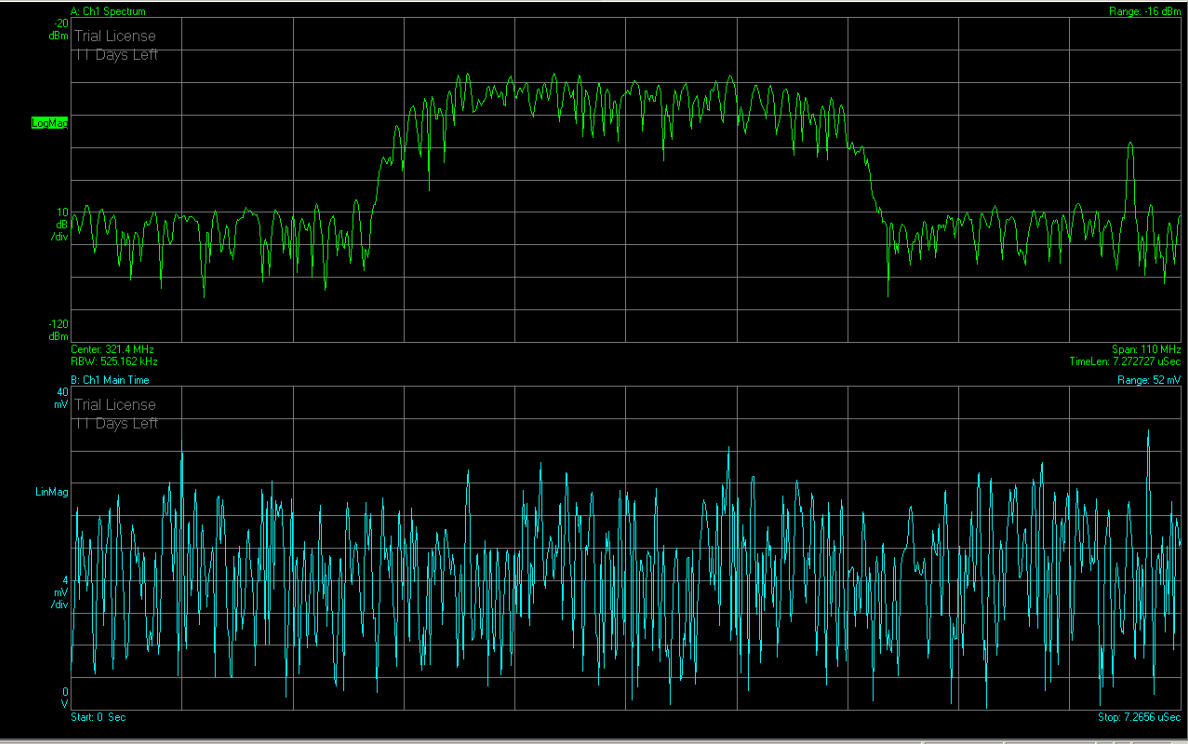
\includegraphics[width=0.9\textwidth]{figures/Aufgabe2_16QAM_1.jpg} 
\caption{Spektrum und zeitlicher Verlauf des empfangenen 16-QAM modulierten Signals}\label{fig:aufg2_16QAM_spec}
\end{figure}

\begin{figure}[H]
\centering
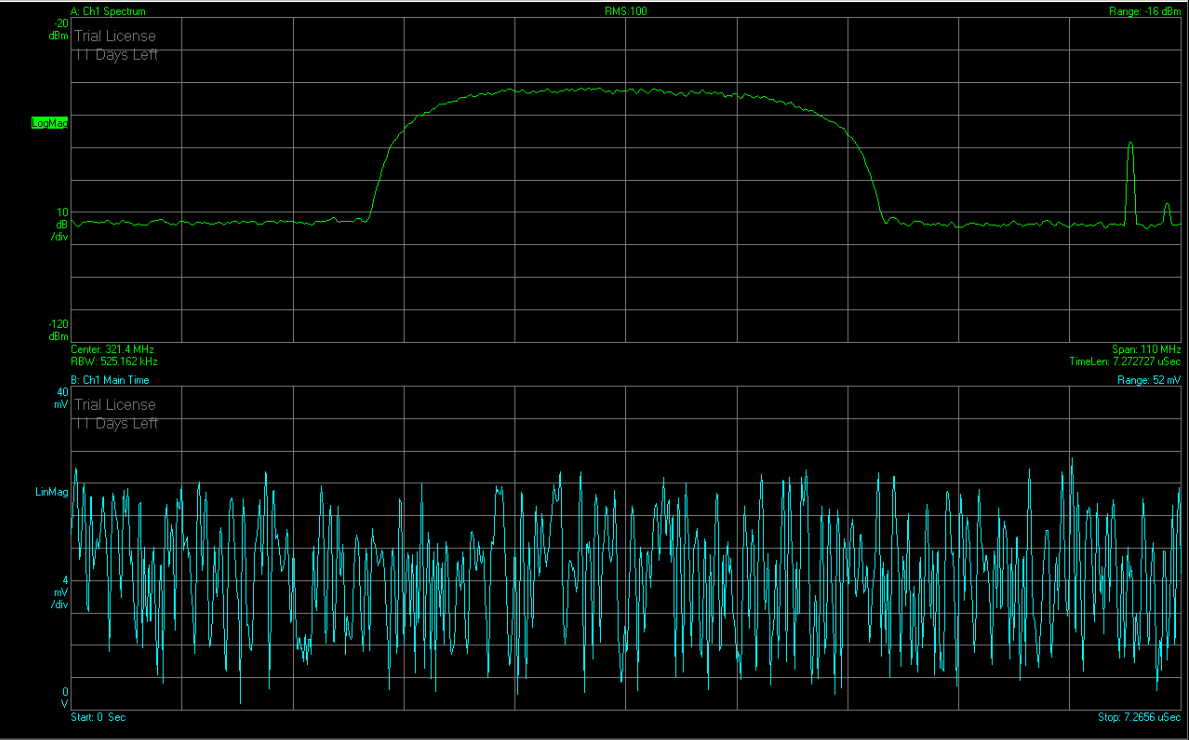
\includegraphics[width=0.9\textwidth]{figures/Aufgabe2_16QAM_avg.jpg} 
\caption{Spektrum und zeitlicher Verlauf des Signals nach dem Glätten.}\label{fig:aufg2_16QAM_spec_avg}
\end{figure}

\pagebreak
\begin{figure}[H]
\centering
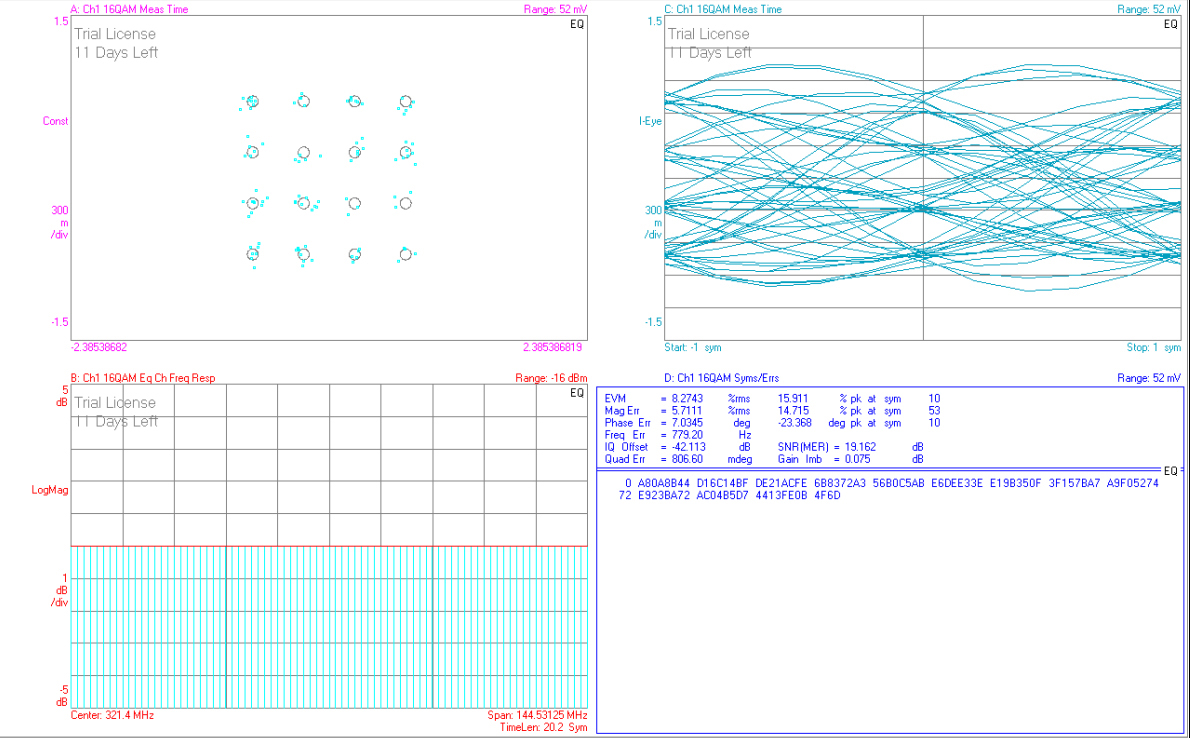
\includegraphics[width=0.9\textwidth]{figures/Aufgabe3_16QAM_demod.jpg} 
\caption{Konstellations- und Augendiagramm des Signals, weiters Amplitudenfrequenzgang des Equalizer und Kanals und Kennwerte zur Beurteilung der Signalqualität}\label{fig:aufg2_16QAM_demod}
\end{figure}

\begin{figure}[H]
\centering
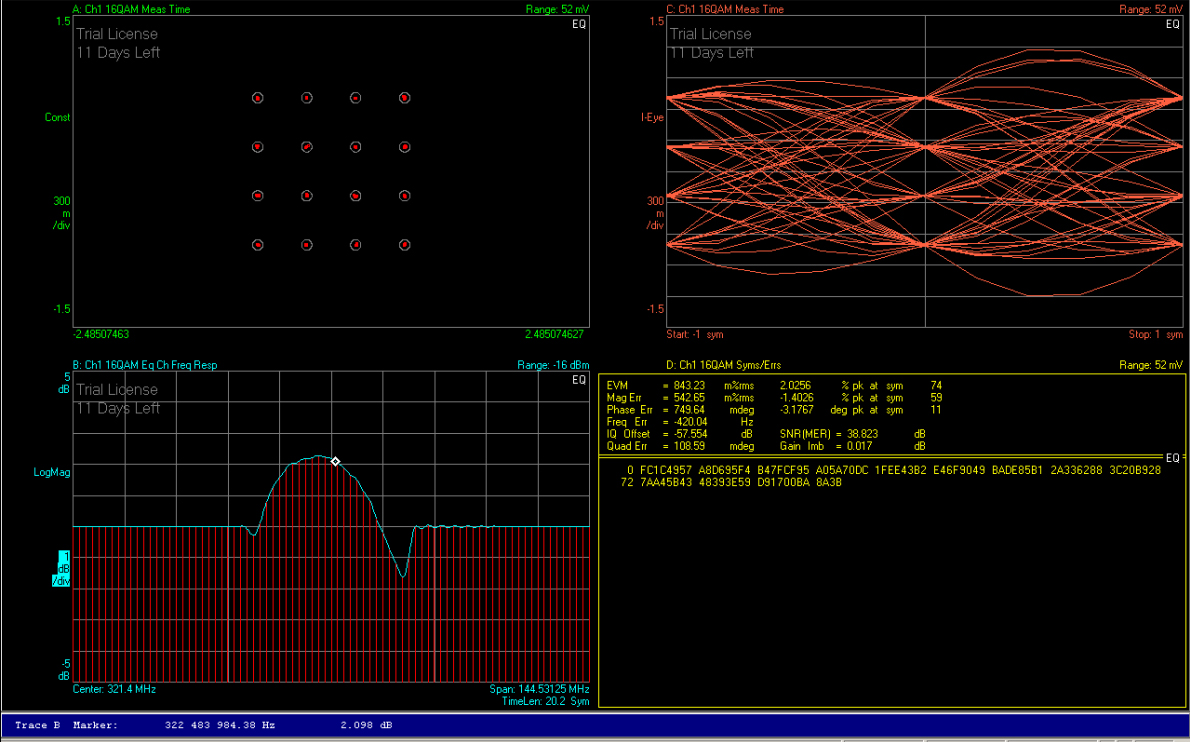
\includegraphics[width=0.9\textwidth]{figures/Aufgabe2_16QAM_demod_equal.jpg} 
\caption{Darstellung wie in Abbildung \ref{fig:aufg2_16QAM_demod}. Im Amplitudenfrequenzgang ist die Anpassung durch den Equalizer zu sehen. }\label{fig:aufg2_16QAM_demod_equal}
\end{figure}


\subsection{Diskussion}
Bei dieser Aufgabenstellung wurden bereitgestellte Daten (breitbandiges Signal), welche laut Aufgabenstellung mittels 16-QAM moduliert und über einen nicht-idealen Kanal mit Bandbegrenzung übertragen worden sind und die entsprechende Konfiguration in die Software \emph{Agilent 89600 Vector Signal Analysis Software} geladen.\\
Wie in Abbildung \ref{fig:aufg2_16QAM_spec} zu sehen, war das Spektrum ziemlich verrauscht. Um das Spektrum leichter interpretieren zu können wurde das Signal mit der Software und den Einstellungen \emph{Average Type RMS (Video)} und \emph{Count 100} \cite[23]{skript} geglättet.\\
In Abbildung \ref{fig:aufg2_16QAM_spec_avg}, in der das geglättete Spektrum zu sehen ist, erkennt man das die Frequenzen über der Mittenfrequenz (321,4 MHz) mehr gedämpft werden als niedrigere Frequenzen. Weiters treten bei ungefähr 370Mhz und 375MHz hochfrequente Störungen auf, welche herausgefilter werden sollten (mittels Filter im Demodulator).\\
Die ungleiche Dämpfung der verschiedenen Frequenzanteile des Signals sind Verzerrungen die durch den nicht-idealen Kanal verursacht werden.\\
\\
Zur demodulation und Darstellung des demodulierten Signals wurde ein andere Konfiguration geladen.\\
In Abbildung \ref{fig:aufg2_16QAM_demod} sind das Konstellationsdiagramm und das Augendiagramm sowie rechts unten Kennwerte zur Signalqualität dargestellt.
Am Konstellationsdiagramm kann man erkennen, das die empfangenen Symbole nicht genau auf den idealen Konstellationspunkten liegen. Die Abweichungen in I-Richtung (Richtung des Anteils des Symbols in Phase) kann man im Augendiagramm ebenfalls sehen (da sich die verschiedenen Übergänge in jeweils Einem der vier Punkte am Abtastzeitpunkt nicht genau schneiden). Diese Abweichungen sind auf die Verzerrung des Signals und Rauschen am Kanal zurück zu führen.\\
Bei den Kennwerten kann man eine Error Vector Magnitude (EVM) von 8,27\%rms und eine Message Error Rate (SNR(MER)) von 19,16db ablesen.\\
\\
In Abbildung \ref{fig:aufg2_16QAM_demod_equal} ist die gleiche Darstellung wie in Abbildung \ref{fig:aufg2_16QAM_demod} zu sehen, aber der Equalizer wurde an den Kanal angepasst und die Verzerrungen wurden damit beseitigt.\\
Die Anpassung des Equalizers wurde von der Software durchgeführt. Dazu musste in den Eigenschaften des Demodulators im Reiter Compensate \emph{Equalization Filter} aktiviert und Adaptive auf \emph{Run} gestellt werden \cite[23]{skript}.
Sobald Adaptive aktiviert war konnte beobachtet werden wie sich der Amplidutenfrequenzgang verändert und die Abweichungen des Signals geringer wurden. Danach wurde Adaptive wieder auf \emph{Hold} gestellt.\\
\\
Im Konstellationsdiagramm, nach der Anpassung des Equalizers, kann man fast keine Abweichungen der empfangenen Symbole gegenüber der idealen Konstellationspunkte sehen. Dies spiegelt auch das Augendiagramm, bei dem sich die Übergänge in den jeweiligen Punkten am Abtastzeitpunkt schneiden, wieder.\\
Die EVM ist durch die Anpassung des Equalizers auf 0,84\%rms gesunken (Verringerung um den Faktor 10) und die SNR(MER) ist auf 38,82db gestiegen (Verbesserung um 19,66db, entspricht zirca einen Faktor von 100).\\
Der Equalizer beseitigt die Verzerrung des Signals durch den Kanal und man kann erkennen, das das Rauschen am Kanal gering war (da nach dem entzerren nur mehr geringe Abweichungen vorhanden sind).\\
\\
Die Übertragungsfunktion des Kanals ist der invertierte Amplitudenfrequenzgang des Equalizers, der in Abbildung \ref{fig:aufg2_16QAM_demod_equal} links unten zu sehen ist.

\pagebreak



\section{Vergleich digitaler Phasenmodulationsverfahren}
\subsection{Aufgabenstellung}
Gegeben ist eine Reihe von Signalen, welche mit unterschiedlichen digitalen Phasenmodulationsverfahren moduliert wurden (QPSK, $\pi/4$-DQPSK, OQPSK, MSK und GMSK). Da es sich um Phasenmodulationsverfahren handelt, sollte die Hüllkurve dieser Signale idealerweise konstant sein. Speziell bei QPSK gibt es aber mitunter starke Einbrüche in der Hüllkurve. Sie sollen nun eine Reihe von Modualtionsverfahren auf ihre Eigenschaften untersuchen. 
\begin{itemize}
\item Demodulieren Sie die Signale und beurteilen Sie die Übergänge zwischen den Symbolen. Diskutieren Sie den Einfluss dieser Übergänge auf die Hüllkurve. 
\item Stellen Sie den Phasenverlauf dar und diskutieren Sie diesen.
\item Finden Sie einen alternativen Weg, Aussagen über die Hüllkurvenschwankungen treffen zu können.
\end{itemize}
\cite[19]{skript}

\subsection{Tabellen}
Es waren keine Tabellen aufzunehmen. 
\subsection{Formeln}
Es wurden keine Formeln benötigt.
\subsection{Berechnungsbeispiele}
Es waren keine Berechnungen durchzuführen.

\pagebreak
\subsection{Diagramme}
\begin{figure}[H]
\centering
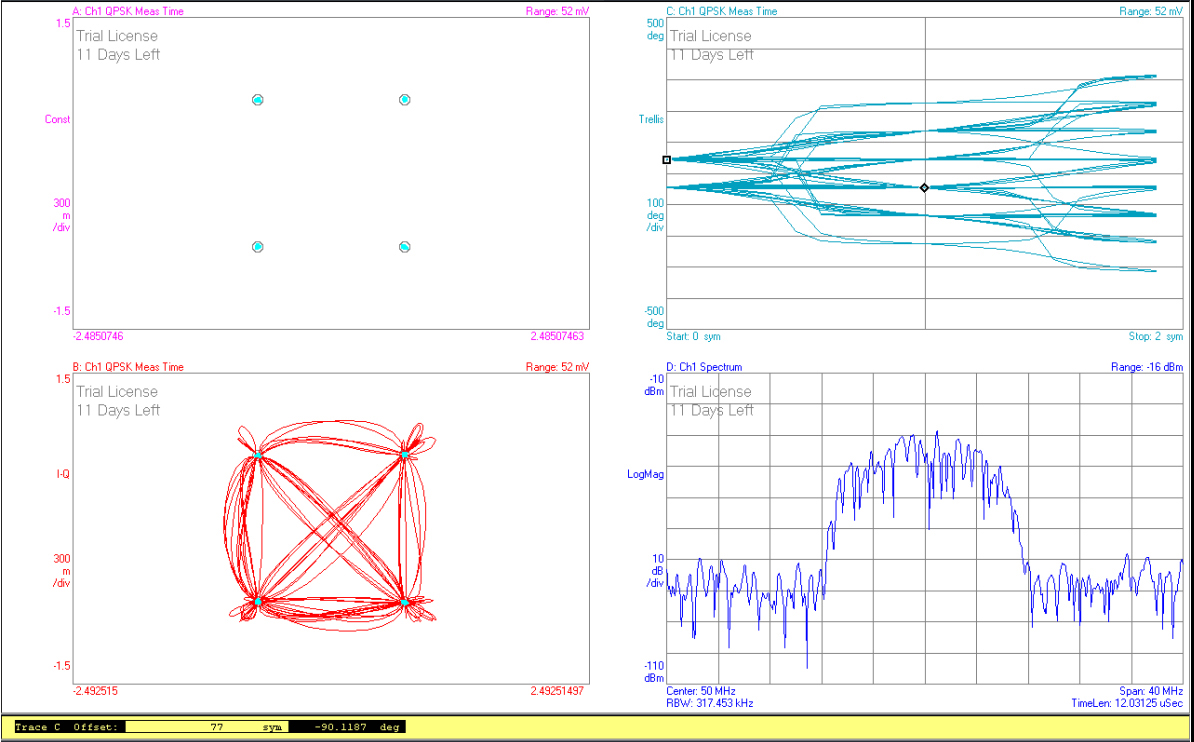
\includegraphics[width=0.9\textwidth]{figures/Aufgabe3_QPSK.jpg} 
\caption{Konstellationsdiagramm, Phasenverlauf, Spektrum eines QPSK modulierten Signals}
\label{fig:3_QPSK}
\end{figure}

\begin{figure}[H]
\centering
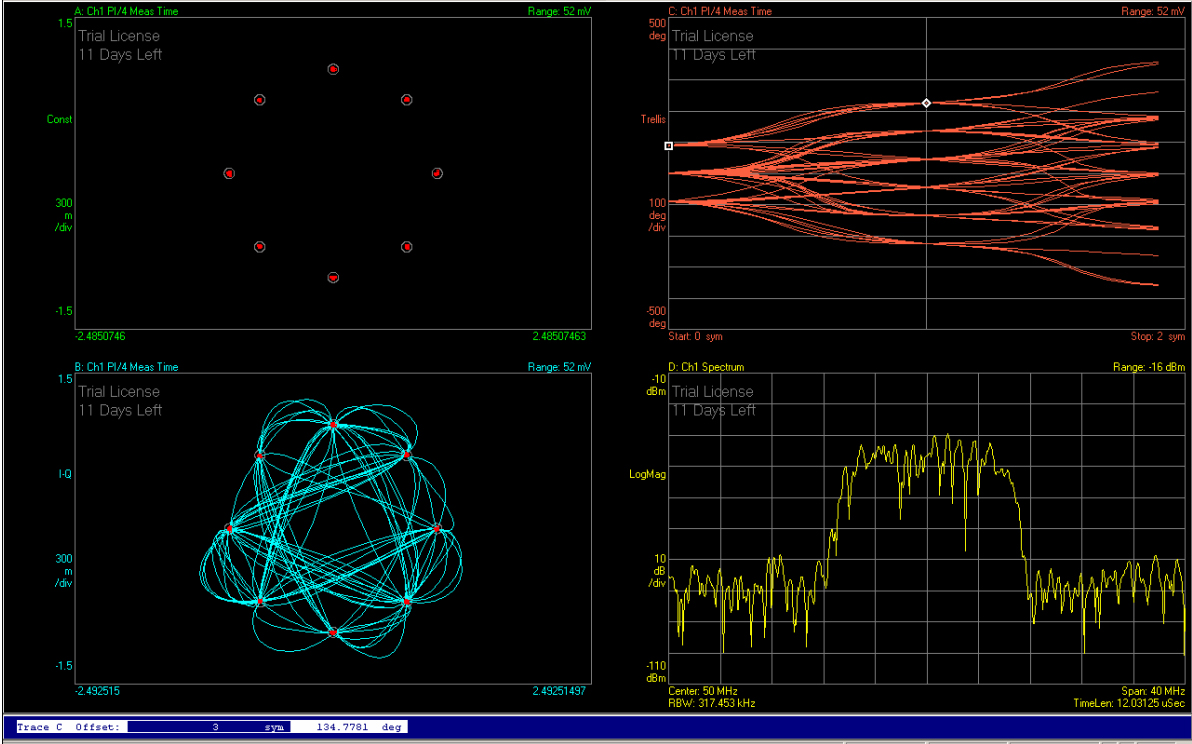
\includegraphics[width=0.9\textwidth]{figures/Aufgabe3_pi4DQPSK.jpg} 
\caption{Konstellationsdiagramm, Phasenverlauf, Spektrum eines $\frac{\pi}{4}$-DQPSK modulierten Signals}
\label{fig:3_PI4DQPSK}
\end{figure}

\begin{figure}[H]
\centering
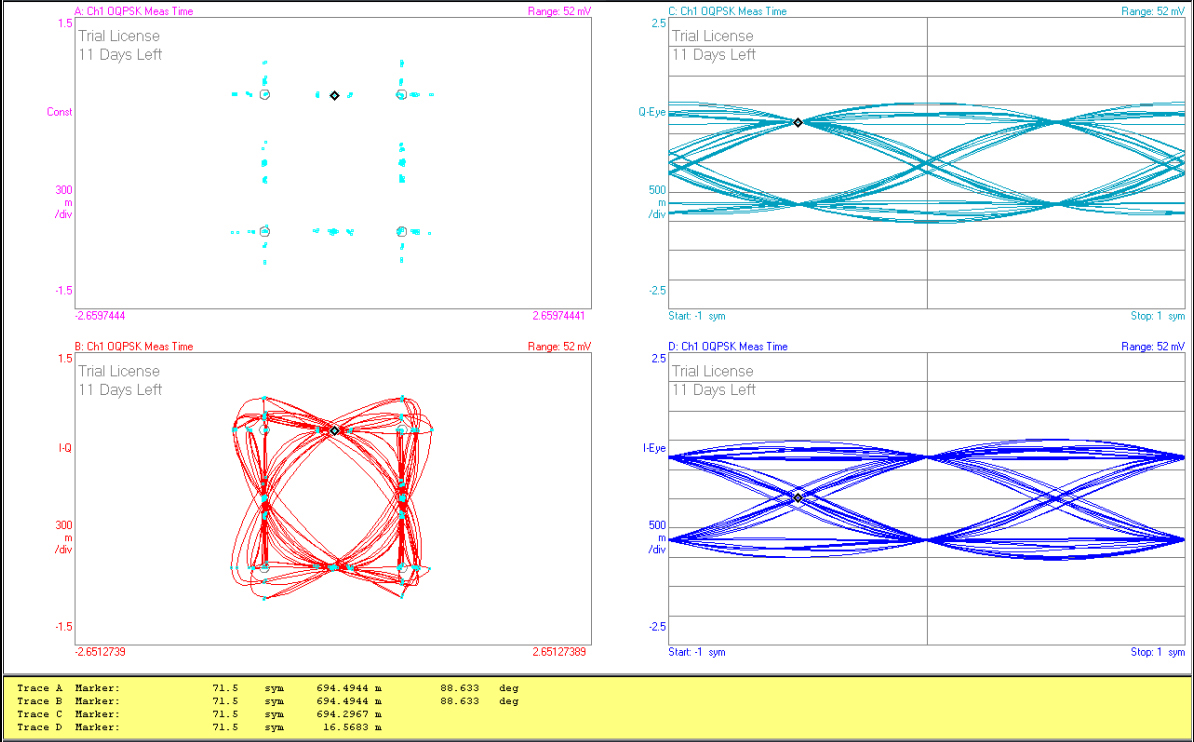
\includegraphics[width=0.9\textwidth]{figures/Aufgabe3_OQPSK.jpg} 
\caption{Konstellationsdiagramm, Augendiagramme eines OQPSK modulierten Signals}
\label{fig:3_OQPSK}
\end{figure}

\pagebreak
\begin{figure}[H]
\centering
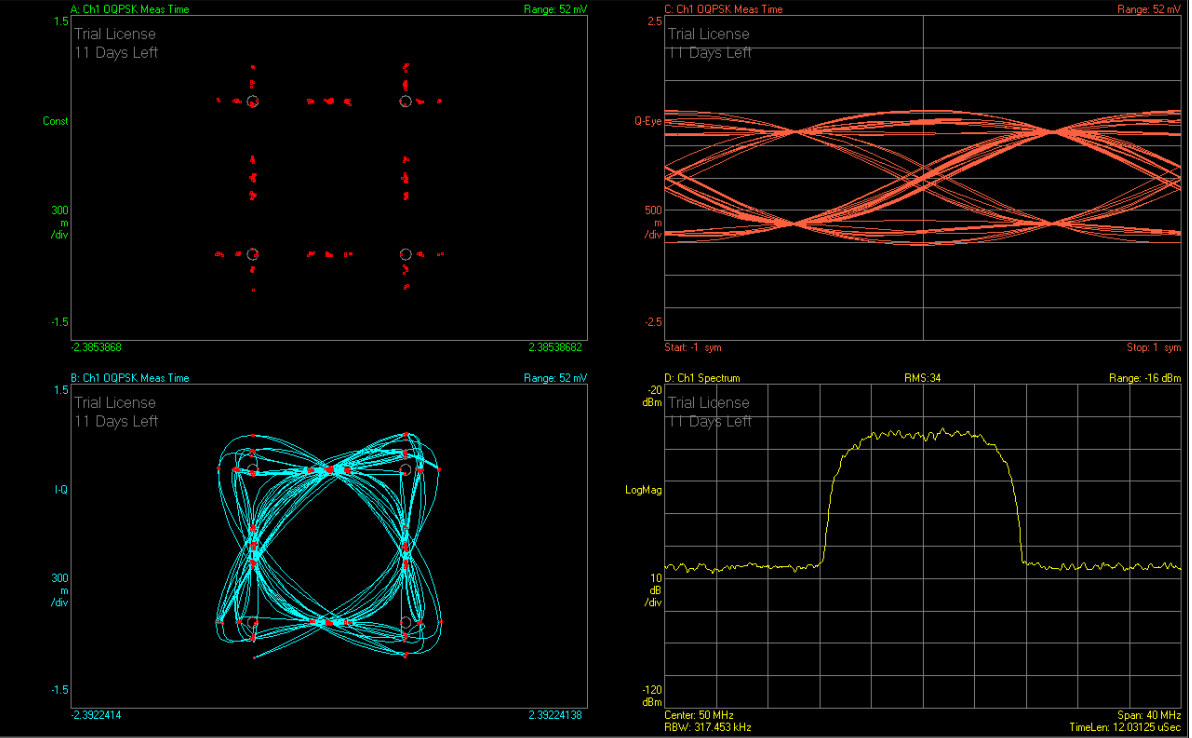
\includegraphics[width=0.9\textwidth]{figures/Aufgabe3_OQPSK_avg.jpg} 
\caption{zusätzliche Darstellung des Spektrums des OQPSK modulierten Signals}
\label{fig:3_OQPSK_spec}
\end{figure}

\begin{figure}[H]
\centering
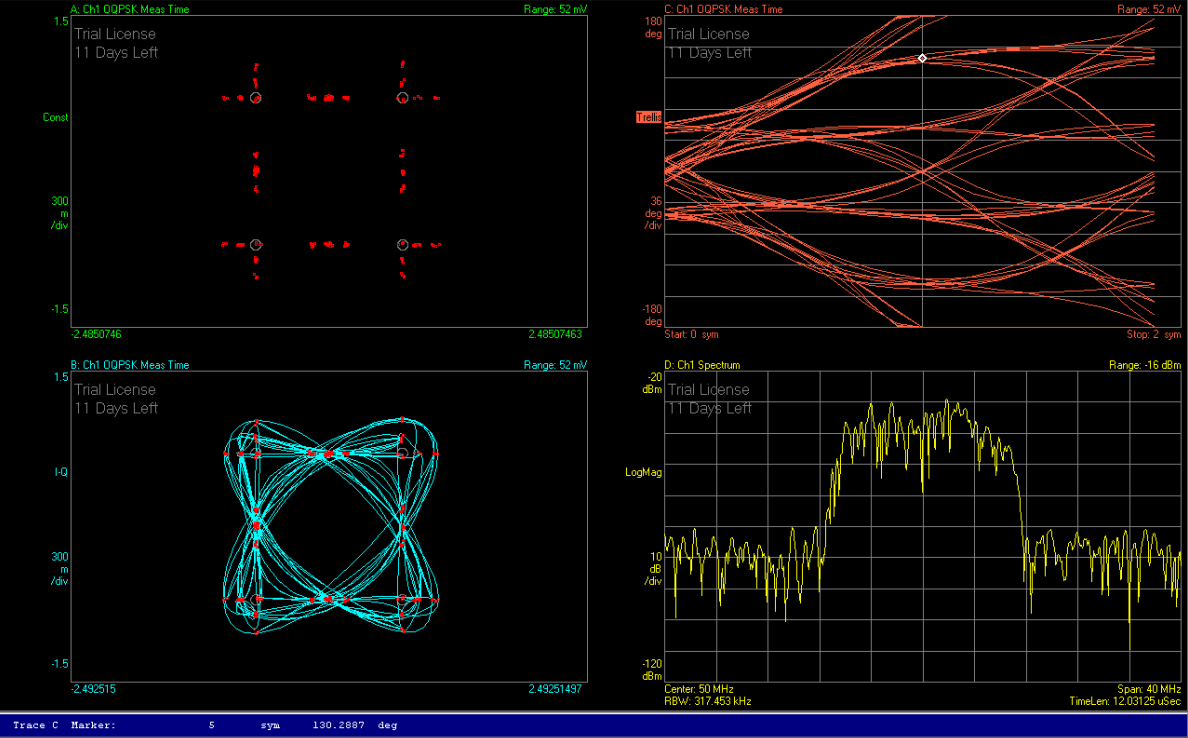
\includegraphics[width=0.9\textwidth]{figures/Aufgabe3_OQPSK_phase.jpg} 
\caption{zusätzliche Darstellung des Phasenverlaufs des OQPSK modulierten Signals}
\label{fig:3_OQPSK_phase}
\end{figure}

\pagebreak
\begin{figure}[H]
\centering
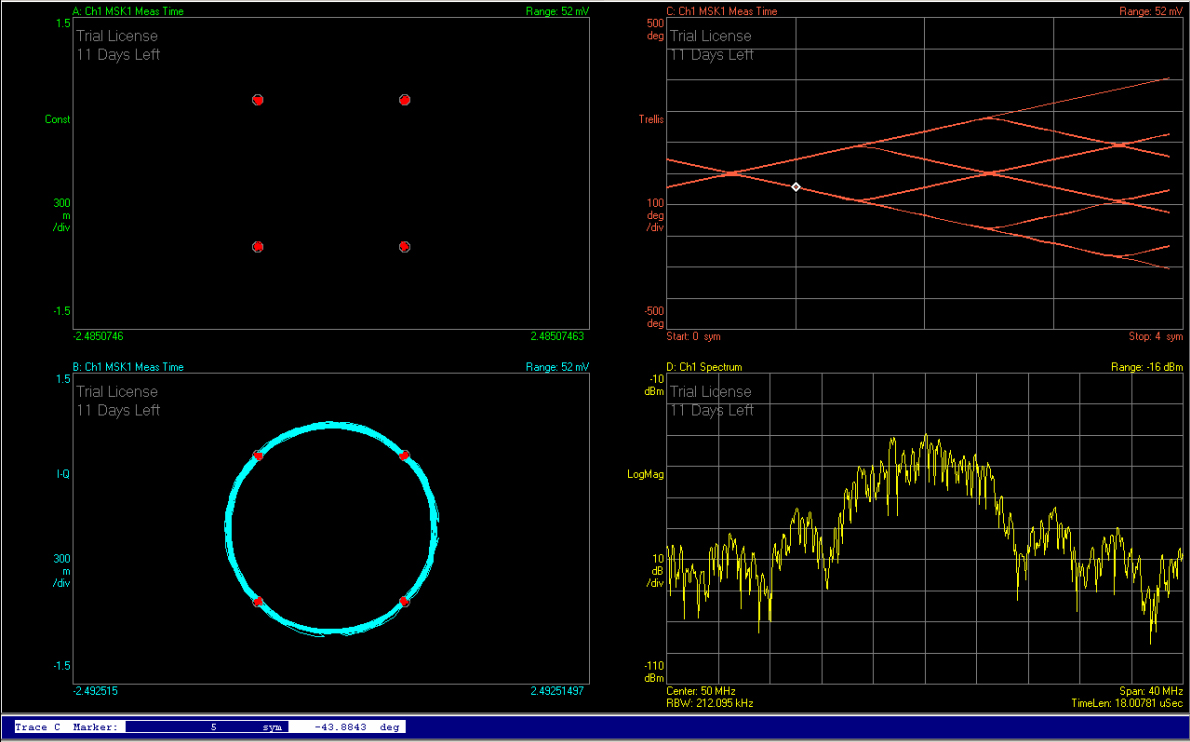
\includegraphics[width=0.9\textwidth]{figures/Aufgabe3_MSK.jpg} 
\caption{Konstellationsdiagramm, Phasenverlauf, Spektrum eines MSK modulierten Signals}
\label{fig:3_MSK}
\end{figure}

\begin{figure}[H]
\centering
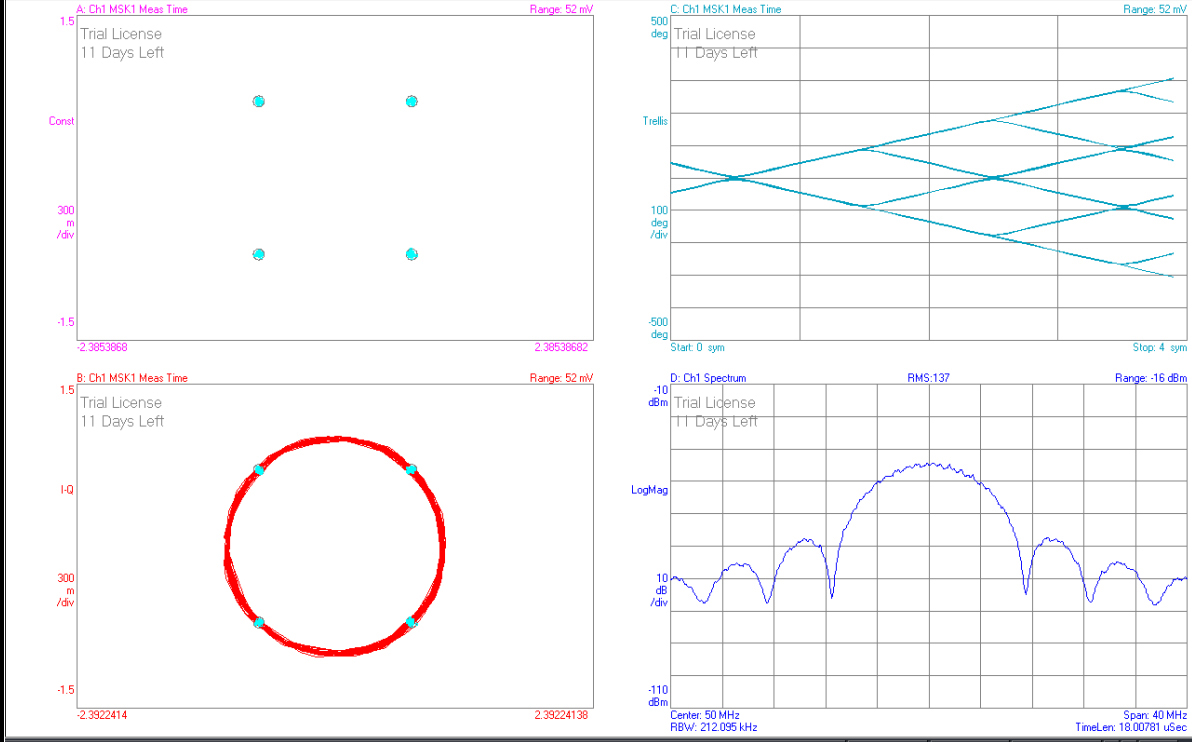
\includegraphics[width=0.9\textwidth]{figures/Aufgabe3_MSK_avg.jpg} 
\caption{Darstellung des geglätteten MSK modulierten Signals}
\label{fig:3_MSK_avg}
\end{figure}

\pagebreak
\begin{figure}[H]
\centering
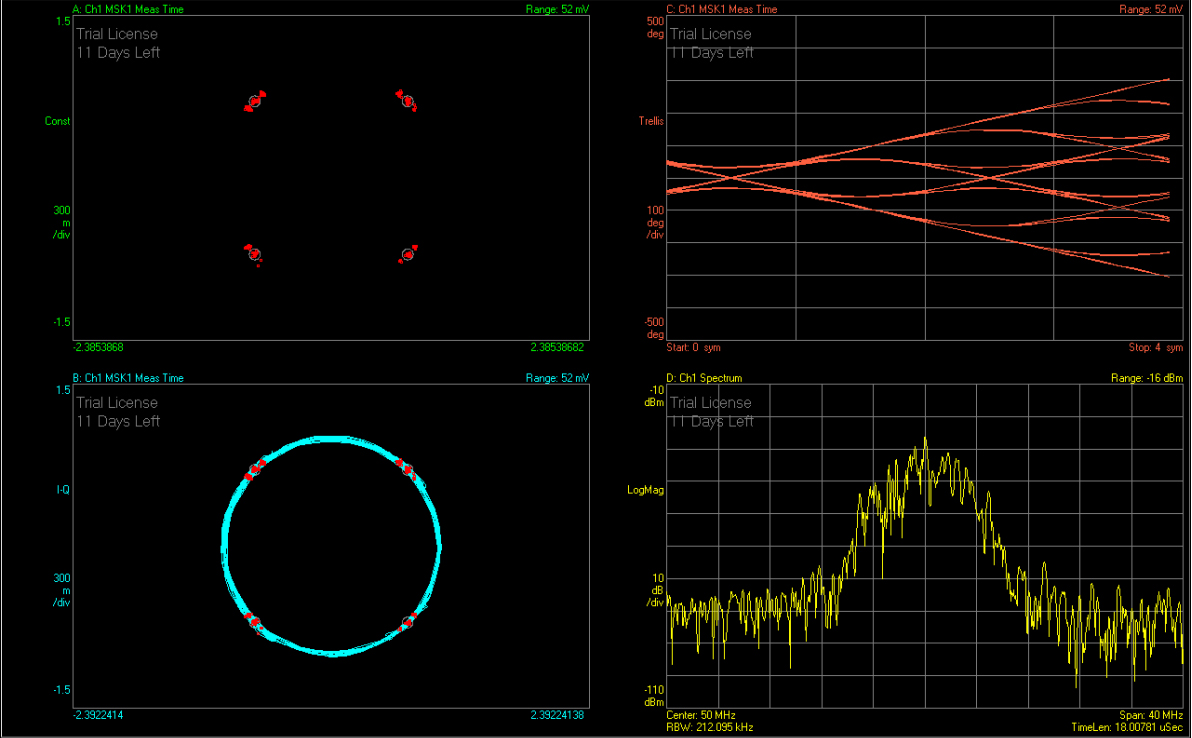
\includegraphics[width=0.9\textwidth]{figures/Aufgabe3_GMSK.jpg} 
\caption{Konstellationsdiagramm, Phasenverlauf, Spektrum eines GMSK modulierten Signals}
\label{fig:3_GMSK}
\end{figure}

\begin{figure}[H]
\centering
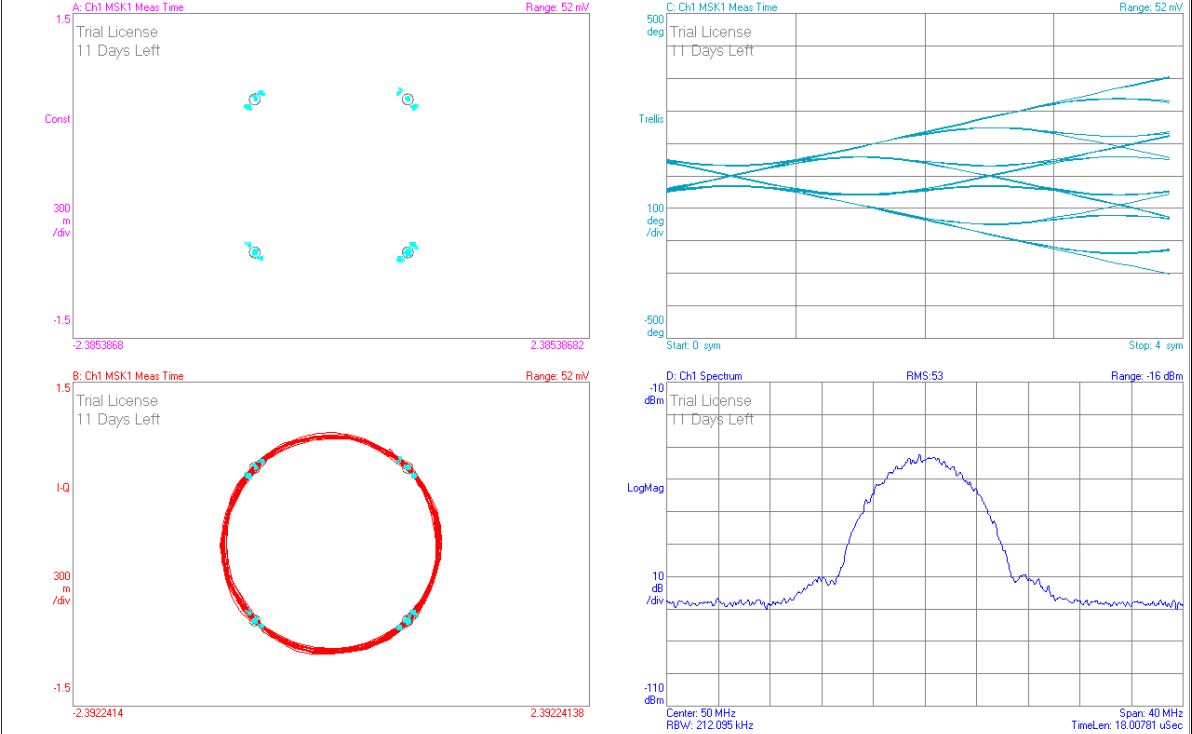
\includegraphics[width=0.9\textwidth]{figures/Aufgabe3_GMSK_avg.jpg} 
\caption{Darstellung des geglätteten GMSK modulierten Signals}
\label{fig:3_GMSK_avg}
\end{figure}

\pagebreak

\subsection{Diskussion}
Bei dieser Aufgabe wurden für jedes Modulationsverfahren eine Datei mit dem Signal und eine oder mehrere Konfigurationsdateien bereitgestellt.\\
In den Abbildungen \ref{fig:3_QPSK} bis \ref{fig:3_GMSK_avg} ist jeweils links unten das I-Q-Diagramm zu sehen. In diesem Diagramm sind die Übergänge zwischen den Symbolen rot aufgetragen. Der Abstand eines Punktes auf der roten Linie zum Koordinatenursprung, welcher in der Mitte des Diagramms liegt, stellt die Amplitude des Signals zu diesem Zeitpunkt dar.\\
Wenn dieser Abstand nicht konstant ist, ist folglich auch die Amplitude des Signals nicht konstant. Wird dieser Abstand zu Null, das heißt der Symbolübergang geht durch den Koordinatenursprung, bricht die Hüllkurve des Signals bis auf Null ein.\\
\\
In den Abbildungen \ref{fig:3_QPSK}, \ref{fig:3_PI4DQPSK} und \ref{fig:3_OQPSK_phase} bis \ref{fig:3_GMSK_avg} ist links oben jeweils ein Trellis-Diagramm zu sehen, in dem man den Phasenverlauf aller Symbolübergänge dieser Modulationsart sehen kann.\\
\\
\begin{itemize}
\item QPSK (Abbildung \ref{fig:3_QPSK}): Es treten Symbolübergänge mit $90^\circ$ und $180^\circ$ Phasensprung auf. Bei $90^\circ$-Sprüngen erkennt man eine Verringerung der Amplitude während des Symbolüberganges, welche einen kleinen Einbruch in der Hüllkurve bewirkt. Bei $180^\circ$-Sprüngen geht der Symbolübergang durch den Koordinatenursprung. Dies bedeutet Einbrüche der Amplitude (Hüllkurve) bis auf Null.\\
Im Trellis-Diagramm sind ebenfalls Phasenänderungen von $0^\circ$, +/-$90^\circ$ und +/-$180^\circ$ von einem Symbol zum nächsten zu erkennen.
\item $\frac{\pi}{4}$-DQPSK (Abbildung \ref{fig:3_PI4DQPSK}): Bei Differential QPSK wird dem Symbol nicht eine bestimmte Phasenlage zugeordnet, sondern die Differenz zweier aufeinander folgender Phasen. Die Phasenzustände kommen bei geraden und ungeraden Abtastzeitpunkten aus unterschiedlichen Phasenräumne. Da diese Räume um  $\frac{\pi}{4}$ gegeneinander gedreht sind, kommen nur noch Phasenübergängen von  $\frac{\pi}{4}$ oder  $\frac{\pi}{4}$ vor. Wie aus Abbildung Abbildung \ref{fig:3_PI4DQPSK} zu erkennen ist, gibt es keine Symbolübergänge die durch den Ursprung gehen. Weiter ist in der Abbildung zu erkennen, dass die Symbolübergänge wie vom Verfahren beschrieben, nur Phasenübergänge $\frac{\pi}{4}$ oder  $\frac{\pi}{4}$ haben und die Hüllkurve nur geringe Veränderungen aufweist. 
\item OQPSK (Abbildungen \ref{fig:3_OQPSK}, \ref{fig:3_OQPSK_spec} und \ref{fig:3_OQPSK_phase}): Da die $180^\circ$-Sprünge bei gleichzeitiger Änderung von I- und Q- Anteilen auftreten, wird bei OQPSK eine Verzögerung von einer halben Symboldauer eingefügt, um diese gleichzeitigen Änderungen zu vermeiden. Dadurch sind nur mehr $90^\circ$-Phasenübergänge möglich. Die Einbrüche in der Hüllkurve sind nicht mehr so problematisch und die Eigenschaften des Spektrums, der Bandbreitenausnutzung und der Bitfehlerhäufigkeit bleiben gleich wie bei QPSK. Wie aus Abbildung \ref{fig:3_OQPSK} entnommen werden kann, gibt es keine $180^\circ$ Phasensprünge mehr (Die Übergänge durch den Ursprung sind weg) und somit ist auch die Änderung der Amplitude nicht mehr so dramatisch. Das in unseren Abbildungen dargestellte Verhalten von OQPSK ergibt sich, da die Q-Phase zwischen zwei idealen Zeitpunkten abgetastet wird. Zu erwarten war eine Abbildung, welche im I/Q-Diagramm so aussieht wie QPSK, nur ohne der $180^\circ$-Sprünge (Linien die durch den Ursprung führen).
\item MSK (Abbildungen \ref{fig:3_MSK} und \ref{fig:3_MSK_avg}): Minimum Shift Keying ist ein Spezialfall der OQPSK. Hierbei werden die Impulse im Basisband durch Sinus-Halbwellen ersetzt. Dadurch werden die Phasenübergänge kontinuierlich und es entstehen keine Phasensprünge mehr, sondern nur Knicke im Phasenverlauf. Wie aus Abbildung \ref{fig:3_MSK_avg} gut zu erkennen ist, bewegen wir uns nur mehr auf dem Kreis entlang, Es gibt keine Sprünge mehr sondern nur leichte Knicke. Im Spektrum ist zu sehen, dass es leichte Nebenkeulen gibt.
\item GMSK (Abbildungen \ref{fig:3_GMSK} und \ref{fig:3_GMSK_avg}): Beim Gaussian Minimum Shift Keying, erlaubt nicht einmal mehr die Knicke die bei MSK entstehen. Das erreicht man indem man nicht Sinus-Halbwellen, sondern gaußförmige Impulse verwendet. Als Parameter für die gaußförmigen Impulse gibt es das Bandbreiten-Zeit-Produkt BT. Wie aus Abbilung \ref{fig:3_MSK_avg} zu entnehmen ist, Sind bei GMSK im Vergleich zu MSK die Nebenkeulen unterdrückt. Die gaußförmigen Impulse sorgen dafür, dass es keine Phasensprünge mehr gibt.
\end{itemize}


\pagebreak



\section{GSM}
\subsection{Aufgabenstellung}
Gegeben ist eine 65ms lange Aufzeichnung aus dem Frequenzbereich von 930-960MHz (oberer Bereich des Downlinks bei GSM 900). Sie sollen in diesem Bereich verschiedene GSM-Kanäle beobachten und ein möglichst starkes Signal demodulieren. Hierzu müssen Sie aufgrund des geringen SNR auf eine genaue Einstellung des Demodulators und des verwendeten Messbereichs achten. 
\begin{itemize}
\item Visualisieren Sie den gegebenen Frequenzbereich mittels Spektrogramm. Suchen Sie einen Kanal, welcher Ihnen zur Untersuchung geeignet erscheint.
\item Versuchen Sie, im Zeitbereich einen Burst zu finden. Versuchen Sie, die GSM Framestruktur zu visualisieren.
\item Stellen Sie den digitalen Demodulator auf die Parameter von GSM ein. Stellen Sie Spektrum, Konstellationsdiagramm und Zeitbereich dar. Diskutieren Sie auch den Phasenverlauf. 
\item Diskutieren Sie die im Skriptum angeführten Parameter von GSM anhand von Spektrum, Spektrogramm, Zeitbereich und digitalem Demodulator. 
\end{itemize}
\cite[19]{skript}

\subsection{Messaufbau}
Es wurde kein Messaufbau benötigt.
\subsection{Tabellen}
Es waren keine Tabellen aufzunehmen. 
\subsection{Formeln}
Es wurden keine Formeln benötigt.
\subsection{Berechnungsbeispiele}
Es wurden keine Berechnungen benötigt.
\pagebreak
\subsection{Diagramme}
\begin{figure}[H]
\centering
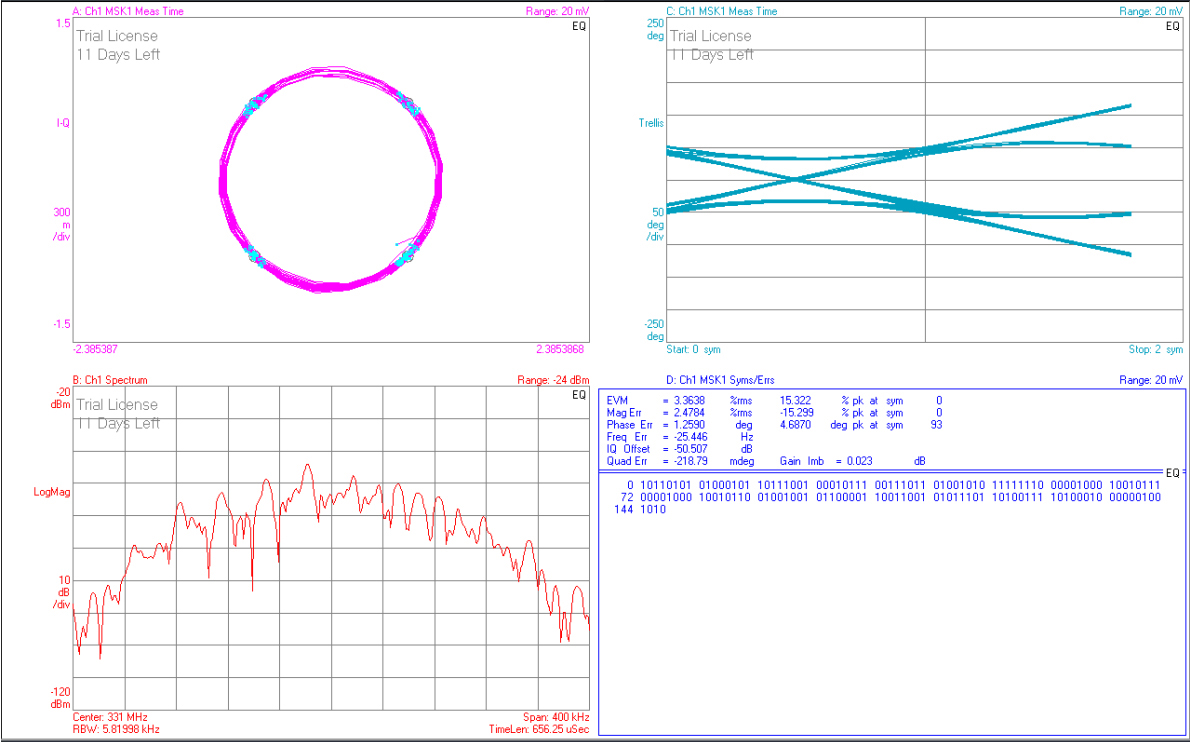
\includegraphics[width=0.9\textwidth]{figures/Aufgabe4_demod.jpg} 
\caption{Konstellationsdiagramm, Trellis-Eye, Spektrum, Kennwerte des demodulierten GSM-Signals}
\label{fig:a4demod}
\end{figure}

\begin{figure}[H]
\centering
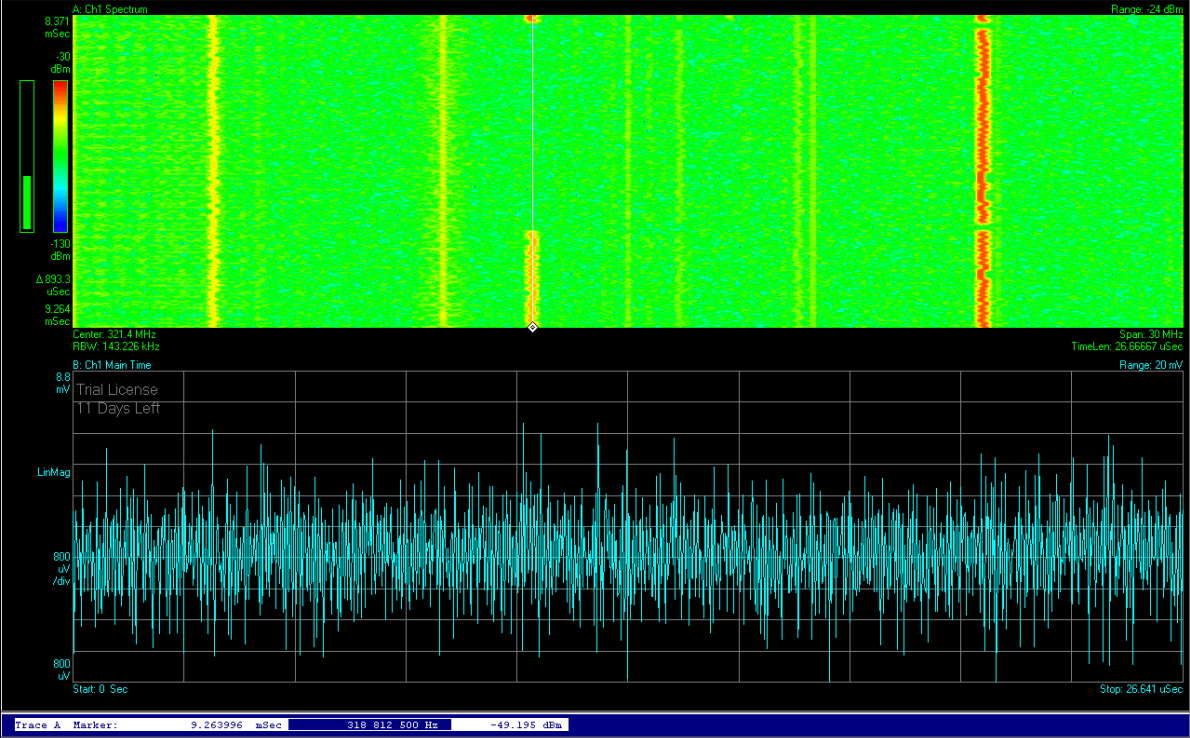
\includegraphics[width=0.9\textwidth]{figures/Aufgabe4_Spektrogramm.jpg} 
\caption{Spektrogramm des GSM-Signals}
\label{fig:spectrogram}
\end{figure}




\subsection{Diskussion}

Im Spektrogramm (Abbildung: \ref{fig:spectrogram}) sind recht deutlich die verschiedenen Kanäle, die auf verschiedene Frequenzen aufgeteilt sind, zu erkennen. Zur Bestimmung der Länge eines Bursts haben wir das Spektrogramm im richtigen Zeitpunkt angehalten. Unsere Messung lieferte als Länge eines Frame-Bursts bei GSM $\approx 800 \mu s$. 

Außerdem ist ersichtlich, dass zwischen den einzelnen Bursts Pausen (Guard Periods) im Spektrogramm sind. Diese sind dazu da, dass es zwischen Übertragungen keine Überschneidungen gibt, da es sonst zu Datenverlust führen würde. Die Guard Periods haben eine zeitliche Dauer von $\approx 30 \mu s$.

Entsprechend der Theorie sollte ein Burst eine Dauer von $576.92 \mu s$ (inklusive Guard Period) besitzen. Der Unterschied ist dadurch zu erklären, dass unsere Methode zur Messung (Spektrogramm anzeigen und im richtigen Zeitpunkt anhalten) sehr ungenau ist.

Der Phasenverlauf von GSM aus Abbildung \ref{fig:a4demod} weist keine Knicke oder Unstetigkeiten auf. Zwischen den Symbolen ändert sich die Phase also stetig, so wie es bei GMSK (Gaussian Minimum Shift Keying) sein sollte. Das Konstellationsdiagramm zeigt, dass die Amplitude der Hüllkurve konstant bleibt, da die Amplitude während den Symbolübergängen gleich groß bleibt (Radius vom Kreis ist konstant).

Das Frequenzspektrum zeigt eine Mittenfrequenz von $331 MHz$ und eine Spanne von $400 kHz$. Aus der Theorie ist bekannt, dass ein Frequenzkanal bei GSM eine Bandbreite von $200 kHz$ besitzt. Im Spektrum aus Abbildung \ref{fig:a4demod} sieht man sehr gut, dass man mit dem verwendeten Modulationsverfahren (GMSK) auch noch Signaleinstreuungen nach der Bandbreite von $200 kHz$ hat. Diese Intersymbolinterferenz wird bei GSM gewollt in kauf genommen.\\

Standardisierte Trägerfrequenzen / Mittenfrequenzen für GSM sind laut Skriptum bei $900 MHz$ bzw. $1800 MHz$. Bei dieser Messung wurde laut Skriptum \cite[19]{skript} das empfangene Signal auf eine Mittenfrequenz von 321,4Mhz transformiert.

Die Einstellungen des digitalen Modulators wurden mit der Konfigurationsdatei mitgeladen. Diese Einstellungen entsprachen den GSM-Werten aus dem Skriptum \cite[17]{skript}.

\begin{thebibliography}{9}

\bibitem{skript}
  Markus Lenzhofer, Paul Meissner, Dr. Klaus Witrisal.
  \emph{Übung E: Messungen an digitalen Übertragungssystemen}.
  Technische Universität Graz.

\end{thebibliography}


 



   
\end{document}